\documentclass[10pt,twocolumn]{article}

\usepackage[margin=0.75in,columnsep=0.3in]{geometry}
\usepackage{times}
\usepackage{amsmath}
\usepackage{graphicx}
\usepackage{caption}
\usepackage{booktabs}
\usepackage{array}
\usepackage[colorlinks=true,citecolor=blue,linkcolor=blue,urlcolor=blue]{hyperref}
\usepackage[compact]{titlesec}
\usepackage{enumitem}
\usepackage{tikz}
\usetikzlibrary{arrows.meta,positioning,calc}
\usepackage{capt-of}

\definecolor{accent}{RGB}{120,30,30}

\setlength{\parindent}{1em}
\setlength{\parskip}{0pt}

\titlespacing*{\section}{0pt}{1.0ex plus .8ex minus .2ex}{.8ex}
\titlespacing*{\subsection}{0pt}{.8ex plus .4ex minus .1ex}{.4ex}
\titleformat{\section}{\normalfont\large\bfseries}{\thesection.}{0.6em}{}
\titleformat{\subsection}{\normalfont\normalsize\bfseries}{\thesubsection}{0.6em}{}

\begin{document}

\twocolumn[
  \begin{center}
    {\LARGE\bfseries Temporal Anti-Aliasing for Single-Photon Reconstruction}\par\vspace{0.8em}
    {\large Adrian Gottwein \quad Limo Kemei \quad Jack Chen \quad Ethan Shao}\par\vspace{0.15em}
    {\small NetIDs: \ttfamily gottwein \quad kkemei \quad zchen848 \quad zshao46}\par\vspace{0.3em}
    {\itshape University of Wisconsin--Madison}\par\vspace{0.6em}
    \small CS 566: Introduction to Computer Vision, Project Proposal \par\vspace{0.2em}
    September 29, 2026
  \end{center}
  \vspace{1.2em}
  \begin{center}
  \begin{minipage}{0.92\textwidth}
  \small
  \textit{Single-photon avalanche diode (SPAD) cameras capture high-speed bursts of binary frames, where each pixel records only whether a photon arrived during a given exposure. A single frame carries almost no usable signal; a clean image only emerges from aligning and merging an entire burst (quanta burst photography). This project investigates single-photon image reconstruction under motion, specifically whether history-rejection heuristics from real-time temporal anti-aliasing (TAA), namely neighborhood clamping and motion-adaptive blending, improve classical align-and-merge reconstruction, particularly under fast motion and disocclusion. We propose to evaluate on the Single Photon Challenge benchmark, co-organized by Prof.\ Gupta's lab, comparing a TAA-augmented pipeline against naive-averaging and hierarchical block-alignment baselines.}
  \end{minipage}
  \end{center}
  \vspace{1.8em}
]

\section{Introduction}

Single-photon avalanche diode (SPAD) cameras capture high-speed bursts of binary frames, where each pixel records only whether a photon arrived during a given exposure. A single frame carries almost no usable signal; a clean image only emerges from aligning and merging an entire burst, a process known as quanta burst photography. We address \textbf{single-photon image reconstruction under motion}: specifically, whether history-rejection heuristics from real-time temporal anti-aliasing (TAA), namely neighborhood clamping and motion-adaptive blending, improve classical align-and-merge reconstruction, especially under fast motion and disocclusion.

This problem matters for two reasons: SPAD arrays are an emerging sensor technology, with megapixel-scale arrays now available, making motion-robust reconstruction increasingly practical; and the standard SPAD pipeline (estimate motion, align, merge) is structurally identical to TAA in real-time rendering, a connection we have not found explored elsewhere.

The project builds directly on Prof.\ Gupta's own quanta burst photography research and the Single Photon Challenge benchmark his lab co-organized, giving the team a public dataset with ground truth rather than requiring custom data collection.

\section{Related Work}

\textbf{Quanta burst photography} (Gupta et al.) establishes the align-then-accumulate pipeline for SPAD bursts that serves as our baseline.

\textbf{Temporal anti-aliasing.} A survey of TAA techniques (Yang et al., NVIDIA, 2020) catalogs the history-rejection methods we adapt to this domain: neighborhood clamping and motion-adaptive blend weights.

\textbf{Single Photon Challenge.} This benchmark provides the dataset and existing leaderboard submissions used for comparison in this work.

\textbf{State of the art.} The current state of the art is the quanta burst photography pipeline: align each binary frame to a reference (block matching or optical flow), then merge by averaging. This works well under static or slow motion, but once alignment becomes unreliable, under fast motion, disocclusion, or low light, misaligned pixels are still blended in at full weight; the pipeline has no mechanism to detect and downweight an untrustworthy alignment, the failure mode we target.

\section{Approach}

We first re-implement the existing quanta burst photography baseline as a validated comparison point, then propose a new approach not previously explored to our knowledge: adapting per-pixel history-rejection heuristics from TAA to explicitly reject unreliable alignments rather than blending them in regardless. Concretely:

\begin{enumerate}[leftmargin=1.4em,itemsep=2pt,topsep=2pt]
  \item Implement a \textit{baseline}: naive frame averaging, followed by hierarchical block alignment and merging (a simplified quanta burst photography pipeline).
  \item Implement a \textit{TAA-augmented pipeline} using the same alignment and merge backbone, adding neighborhood-clamping history rejection, motion-adaptive blend weights, and a per-pixel confidence map.
  \item Evaluate both pipelines on held-out Single Photon Challenge training scenes and on synthetic motion sweeps generated with the visionsim simulator.
  \item Analyze where and why each method breaks down under fast motion and disocclusion.
\end{enumerate}

Figure~\ref{fig:pipeline} illustrates the per-frame mechanism of the TAA-augmented pipeline and the point at which the naive-averaging baseline diverges from it. This approach draws on course material including image alignment and transformations, RANSAC, optical flow, tracking, and the quanta computational imaging lecture.

\begin{figure*}[t]
\centering
{\sffamily
\resizebox{\textwidth}{!}{%
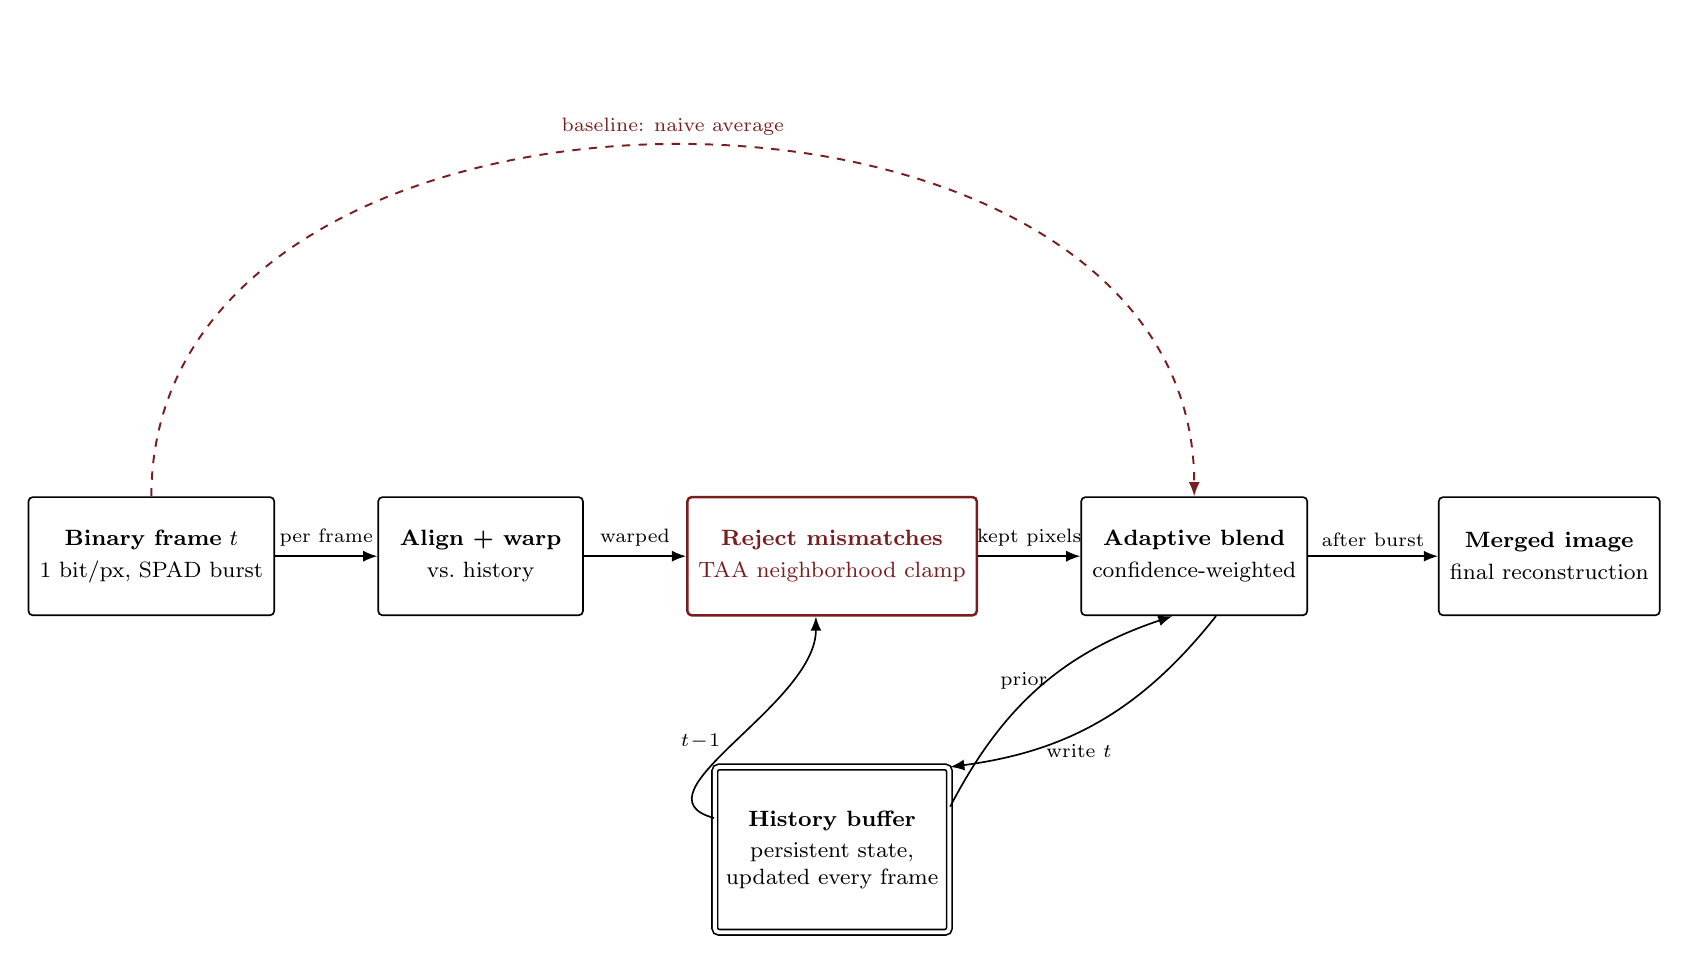
\begin{tikzpicture}[
  font=\footnotesize,
  block/.style={
    rectangle, draw=black, line width=0.6pt, rounded corners=1.5pt,
    minimum width=2.6cm, minimum height=1.5cm, align=center, inner sep=4pt
  },
  hl/.style={block, draw=accent, line width=0.9pt},
  state/.style={
    rectangle, draw=black, line width=0.6pt, rounded corners=1.5pt,
    minimum width=2.6cm, minimum height=2.1cm, align=center, inner sep=4pt,
    double, double distance=1.4pt
  },
  arr/.style={-{Latex[length=1.8mm,width=1.4mm]}, line width=0.6pt},
  lbl/.style={font=\scriptsize, align=center},
]

\node[block] (A) at (0,0) {\textbf{Binary frame} $t$\\[2pt]\footnotesize 1 bit/px, SPAD burst};
\node[block, right=1.3cm of A] (B) {\textbf{Align + warp}\\[2pt]\footnotesize vs.\ history};
\node[hl,   right=1.3cm of B] (E) {\textbf{\textcolor{accent}{Reject mismatches}}\\[2pt]\footnotesize\textcolor{accent}{TAA neighborhood clamp}};
\node[block, right=1.3cm of E] (F) {\textbf{Adaptive blend}\\[2pt]\footnotesize confidence-weighted};
\node[block, right=1.65cm of F] (G) {\textbf{Merged image}\\[2pt]\footnotesize final reconstruction};

\draw[arr] (A) -- (B) node[midway, above, lbl] {per frame};
\draw[arr] (B) -- (E) node[midway, above, lbl] {warped};
\draw[arr] (E) -- (F) node[midway, above, lbl] {kept pixels};
\draw[arr] (F) -- (G) node[midway, above, lbl] {after burst};

\node[state, below=1.9cm of E] (D) {\textbf{History buffer}\\[2pt]\footnotesize persistent state,\\ updated every frame};

\draw[arr] (D.165) to[out=165,in=-90] node[left=1pt, lbl] {$t\!-\!1$} (E.-105);
\draw[arr] (D.20)  to[bend left=22] node[pos=0.42, above=1pt, lbl] {prior} (F.-110);
\draw[arr] (F.-70) to[bend left=22] node[pos=0.58, below=1pt, lbl] {write $t$} (D.35);

\draw[arr, dashed, draw=accent, line width=0.7pt]
  (A.north) to[out=90, in=90, looseness=1.15]
  node[midway, above, lbl, text=accent] {baseline: naive average}
  (F.north);

\end{tikzpicture}%
}}
\caption{Per frame, the TAA-augmented pipeline (solid) warps the incoming binary frame to align with the running history buffer, rejects pixels where that alignment is unreliable, and adaptively blends the rest back into the history, which feeds the next frame and, after the full burst, the final reconstruction. The naive-averaging baseline (dashed) instead accumulates every frame directly, with no alignment or rejection.}
\label{fig:pipeline}
\end{figure*}

We expect the TAA-augmented pipeline to outperform the baseline in the fast-motion and disocclusion regime, where naive blending is most error-prone. The neighborhood clamp checks whether the aligned history agrees with the incoming frame's local neighborhood and rejects the pixel when it does not; the baseline has no analogous mechanism and blends every aligned pixel at a fixed or naively motion-scaled weight regardless of trustworthiness. Since both pipelines share the same alignment and merge backbone, any difference in quality is attributable to history-rejection alone.

\section{Data}

The Single Photon Challenge dataset provides 50 simulated training scenes and 5 test scenes (ground truth withheld), each burst (a ``photon cube'') consisting of 1{,}024 binary frames. The full set is approximately 425~GB; we will work with a 5--10 chunk subset (roughly 8.5~GB per chunk), supplemented with our own synthetic motion sweeps generated via the MIT-licensed visionsim simulator.

\begin{figure}[h]
\centering
\includegraphics[width=0.4\columnwidth]{result-baseline.png}\hfill
\includegraphics[width=0.4\columnwidth]{result-groundtruth.png}
\caption{Preliminary result: baseline reconstruction (left) vs.\ ground truth (right), confirming the data pipeline and baseline already work.}
\label{fig:prelim}
\end{figure}

\section{Evaluation Plan}

We will report PSNR and SSIM on held-out training scenes, and conduct a failure analysis against motion speed using visionsim sweeps to characterize when temporal reconstruction breaks down. The contribution is framed as an interpretable classical method with a rigorous failure analysis, rather than a state-of-the-art claim against neural approaches.

\section{Scope and Feasibility}

This project topic was discussed with Prof.\ Gupta, who confirmed it is a reasonable and worthwhile direction. As expected at this stage, scope may be refined as implementation progresses. Prof.\ Gupta also offered to connect the team with his lab for data access or implementation guidance if needed.

\section{Timeline}

\begingroup
\centering
\small
\renewcommand{\arraystretch}{0.9}
\begin{tabular}{@{}p{0.08\columnwidth}p{0.30\columnwidth}p{0.52\columnwidth}@{}}
\toprule
\textbf{Wk} & \textbf{Dates} & \textbf{Milestone} \\
\midrule
1--2 & Sep 29--Oct 12 & Data pipeline and baseline working \\
3--4 & Oct 13--Oct 26 & TAA-augmented pipeline implemented \\
5 & Oct 27--Oct 29 & Mid-term report: baseline vs.\ TAA \\
6--8 & Oct 30--Nov 19 & Motion sweeps, failure analysis \\
9 & Nov 20--Nov 30 & Final evaluation, ablations \\
10 & Dec 1--Dec 10 & Presentation and final webpage \\
\bottomrule
\end{tabular}
\captionof{table}{Project timeline by course week.}
\label{tab:timeline}
\endgroup

\end{document}
